\documentclass{ximera}

 

\usepackage{epsfig}

\graphicspath{
  {./}
  {figures/}
}

\usepackage{morewrites}
\makeatletter
\newcommand\subfile[1]{%
\renewcommand{\input}[1]{}%
\begingroup\skip@preamble\otherinput{#1}\endgroup\par\vspace{\topsep}
\let\input\otherinput}
\makeatother

\newcommand{\includeexercises}{\directlua{dofile("/home/jim/linearAlgebra/laode/exercises.lua")}}

%\newcounter{ccounter}
%\setcounter{ccounter}{1}
%\newcommand{\Chapter}[1]{\setcounter{chapter}{\arabic{ccounter}}\chapter{#1}\addtocounter{ccounter}{1}}

%\newcommand{\section}[1]{\section{#1}\setcounter{thm}{0}\setcounter{equation}{0}}

%\renewcommand{\theequation}{\arabic{chapter}.\arabic{section}.\arabic{equation}}
%\renewcommand{\thefigure}{\arabic{chapter}.\arabic{figure}}
%\renewcommand{\thetable}{\arabic{chapter}.\arabic{table}}

%\newcommand{\Sec}[2]{\section{#1}\markright{\arabic{ccounter}.\arabic{section}.#2}\setcounter{equation}{0}\setcounter{thm}{0}\setcounter{figure}{0}}

\newcommand{\Sec}[2]{\section{#1}}

\setcounter{secnumdepth}{2}
%\setcounter{secnumdepth}{1} 

%\newcounter{THM}
%\renewcommand{\theTHM}{\arabic{chapter}.\arabic{section}}

\newcommand{\trademark}{{R\!\!\!\!\!\bigcirc}}
%\newtheorem{exercise}{}

\newcommand{\dfield}{{\sf dfield9}}
\newcommand{\pplane}{{\sf pplane9}}

\newcommand{\EXER}{\section*{Exercises}}%\vspace*{0.2in}\hrule\small\setcounter{exercise}{0}}
\newcommand{\CEXER}{}%\vspace{0.08in}\begin{center}Computer Exercises\end{center}}
\newcommand{\TEXER}{} %\vspace{0.08in}\begin{center}Hand Exercises\end{center}}
\newcommand{\AEXER}{} %\vspace{0.08in}\begin{center}Hand Exercises\end{center}}

% BADBAD: \newcommand{\Bbb}{\bf}

\newcommand{\R}{\mbox{$\Bbb{R}$}}
\newcommand{\C}{\mbox{$\Bbb{C}$}}
\newcommand{\Z}{\mbox{$\Bbb{Z}$}}
\newcommand{\N}{\mbox{$\Bbb{N}$}}
\newcommand{\D}{\mbox{{\bf D}}}
\usepackage{amssymb}
%\newcommand{\qed}{\hfill\mbox{\raggedright$\square$} \vspace{1ex}}
%\newcommand{\proof}{\noindent {\bf Proof:} \hspace{0.1in}}

\newcommand{\setmin}{\;\mbox{--}\;}
\newcommand{\Matlab}{{M\small{AT\-LAB}} }
\newcommand{\Matlabp}{{M\small{AT\-LAB}}}
\newcommand{\computer}{\Matlab Instructions}
\newcommand{\half}{\mbox{$\frac{1}{2}$}}
\newcommand{\compose}{\raisebox{.15ex}{\mbox{{\scriptsize$\circ$}}}}
\newcommand{\AND}{\quad\mbox{and}\quad}
\newcommand{\vect}[2]{\left(\begin{array}{c} #1_1 \\ \vdots \\
 #1_{#2}\end{array}\right)}
\newcommand{\mattwo}[4]{\left(\begin{array}{rr} #1 & #2\\ #3
&#4\end{array}\right)}
\newcommand{\mattwoc}[4]{\left(\begin{array}{cc} #1 & #2\\ #3
&#4\end{array}\right)}
\newcommand{\vectwo}[2]{\left(\begin{array}{r} #1 \\ #2\end{array}\right)}
\newcommand{\vectwoc}[2]{\left(\begin{array}{c} #1 \\ #2\end{array}\right)}

\newcommand{\ignore}[1]{}


\newcommand{\inv}{^{-1}}
\newcommand{\CC}{{\cal C}}
\newcommand{\CCone}{\CC^1}
\newcommand{\Span}{{\rm span}}
\newcommand{\rank}{{\rm rank}}
\newcommand{\trace}{{\rm tr}}
\newcommand{\RE}{{\rm Re}}
\newcommand{\IM}{{\rm Im}}
\newcommand{\nulls}{{\rm null\;space}}

\newcommand{\dps}{\displaystyle}
\newcommand{\arraystart}{\renewcommand{\arraystretch}{1.8}}
\newcommand{\arrayfinish}{\renewcommand{\arraystretch}{1.2}}
\newcommand{\Start}[1]{\vspace{0.08in}\noindent {\bf Section~\ref{#1}}}
\newcommand{\exer}[1]{\noindent {\bf \ref{#1}}}
\newcommand{\ans}{}
\newcommand{\matthree}[9]{\left(\begin{array}{rrr} #1 & #2 & #3 \\ #4 & #5 & #6
\\ #7 & #8 & #9\end{array}\right)}
\newcommand{\cvectwo}[2]{\left(\begin{array}{c} #1 \\ #2\end{array}\right)}
\newcommand{\cmatthree}[9]{\left(\begin{array}{ccc} #1 & #2 & #3 \\ #4 & #5 &
#6 \\ #7 & #8 & #9\end{array}\right)}
\newcommand{\vecthree}[3]{\left(\begin{array}{r} #1 \\ #2 \\
#3\end{array}\right)}
\newcommand{\cvecthree}[3]{\left(\begin{array}{c} #1 \\ #2 \\
#3\end{array}\right)}
\newcommand{\cmattwo}[4]{\left(\begin{array}{cc} #1 & #2\\ #3
&#4\end{array}\right)}

\newcommand{\Matrix}[1]{\ensuremath{\left(\begin{array}{rrrrrrrrrrrrrrrrrr} #1 \end{array}\right)}}

\newcommand{\Matrixc}[1]{\ensuremath{\left(\begin{array}{cccccccccccc} #1 \end{array}\right)}}



\renewcommand{\labelenumi}{\theenumi)}
\newenvironment{enumeratea}%
{\begingroup
 \renewcommand{\theenumi}{\alph{enumi}}
 \renewcommand{\labelenumi}{(\theenumi)}
 \begin{enumerate}}
 {\end{enumerate}\endgroup}



\newcounter{help}
\renewcommand{\thehelp}{\thesection.\arabic{equation}}

%\newenvironment{equation*}%
%{\renewcommand\endequation{\eqno (\theequation)* $$}%
%   \begin{equation}}%
%   {\end{equation}\renewcommand\endequation{\eqno \@eqnnum
%$$\global\@ignoretrue}}

%\input{psfig.tex}

\author{Martin Golubitsky and Michael Dellnitz}

%\newenvironment{matlabEquation}%
%{\renewcommand\endequation{\eqno (\theequation*) $$}%
%   \begin{equation}}%
%   {\end{equation}\renewcommand\endequation{\eqno \@eqnnum
% $$\global\@ignoretrue}}

\newcommand{\soln}{\textbf{Solution:} }
\newcommand{\exercap}[1]{\centerline{Figure~\ref{#1}}}
\newcommand{\exercaptwo}[1]{\centerline{Figure~\ref{#1}a\hspace{2.1in}
Figure~\ref{#1}b}}
\newcommand{\exercapthree}[1]{\centerline{Figure~\ref{#1}a\hspace{1.2in}
Figure~\ref{#1}b\hspace{1.2in}Figure~\ref{#1}c}}
\newcommand{\para}{\hspace{0.4in}}

\renewenvironment{solution}{\suppress}{\endsuppress}

\ifxake
\newenvironment{matlabEquation}{\begin{equation}}{\end{equation}}
\else
\newenvironment{matlabEquation}%
{\let\oldtheequation\theequation\renewcommand{\theequation}{\oldtheequation*}\begin{equation}}%
  {\end{equation}\let\theequation\oldtheequation}
\fi

\makeatother


\title{c1.tex}

\begin{document}
\begin{abstract}
BADBAD
\end{abstract}
\maketitle

\setcounter{page}{1}
%\setcounter{ccounter}{0}

\chapter{Preliminaries}
\label{chap:prelim}

The subjects of linear algebra and differential equations involve
manipulating vector equations.  In this chapter we introduce our
notation for vectors and matrices --- and we introduce \Matlabp,
a computer program that is designed to perform vector
manipulations in a natural way.

We begin, in Section~\ref{S:1.1}, by defining vectors and matrices, and
by explaining how to add and scalar multiply vectors and matrices.
In Section~\ref{S:1.2} we explain how to enter vectors and matrices
into \Matlabp, and how to perform the operations of addition and
scalar multiplication in \Matlabp.  There are many special types of matrices;
these types are introduced in Section~\ref{S:1.3}. In the concluding
section, we introduce the geometric interpretations of vector addition
and scalar multiplication; in addition we discuss the angle between
vectors through the use of the dot product of two vectors.


\section{Vectors and Matrices}
\label{S:1.1}

In their elementary form, matrices and vectors are just lists of 
real numbers in different formats.  An $n$-vector is a list of $n$ 
numbers $(x_1,x_2,\ldots,x_n)$.  We may write this vector as a 
{\em row\/} vector\index{vector} as we have just done --- or as a 
{\em column\/} vector
\[
\vect{x}{n}.
\]
The set of all (real-valued) $n$-vectors is denoted by $\R^n$\index{$\R^n$}; 
so points in $\R^n$ are called vectors.  The sets $\R^n$ when $n$ is small
are very familiar sets.  The set $\R^1=\R$ is the real number
line, and the set $\R^2$ is the Cartesian plane\index{Cartesian plane}.
The set $\R^3$ consists of points or vectors in three dimensional space.

An $m\times n$ {\em matrix\/}\index{matrix} is a rectangular array
of numbers with $m$ rows and $n$ columns.  A general $2\times 3$
matrix has the form
\[
A=\left(\begin{array}{ccc} a_{11} & a_{12} & a_{13} \\
     a_{21} & a_{22} & a_{23} \end{array}\right).
\]
We use the convention that matrix entries $a_{ij}$ are indexed
so that the first subscript $i$ refers to the {\em row\/}
\index{row} while the second subscript $j$ refers to the {\em
column\/}\index{column}.  So the entry $a_{21}$ refers to the
matrix entry in the $2^{nd}$ row, $1^{st}$ column.

An $n\times m$ matrix $A$ and an $n'\times m'$ matrix $B$ are equal
precisely when the sizes of the matrices are equal ($n=n'$ and $m=m'$)
and when each of the corresponding entries are equal ($a_{ij}=b_{ij}$).

There is some redundancy in the use of the terms ``vector'' and
``matrix''.  For example, a row $n$-vector may be thought of as a 
$1\times n$ matrix, and a column $n$-vector may be thought of as a 
$n\times 1$ matrix.  There are situations where matrix notation is 
preferable to vector notation and vice-versa.


\subsection*{Addition and Scalar Multiplication of Vectors}

There are two basic operations on vectors: addition and scalar
multiplication.  Let $x=(x_1,\ldots,x_n)$ and
$y=(y_1,\ldots,y_n)$ be $n$-vectors.  Then
\[
x+y=(x_1+y_1,\ldots,x_n+y_n);
\]
that is, {\em vector addition\/}\index{vector!addition} is
defined as componentwise addition.

Similarly, {\em scalar multiplication\/}\index{scalar multiplication}
is defined as
componentwise multiplication.  A {\em scalar\/} is just a
number. Initially, we use the term scalar\index{scalar} to refer to a real
number --- but later on we sometimes use the term scalar
to refer to a {\em complex\/} number.  Suppose $r$ is a real
number; then the multiplication of a vector by the scalar $r$
is defined as
\[
rx = (rx_1,\ldots,rx_n).
\]

Subtraction of vectors\index{vector!subtraction} is defined simply as
\[
x-y = (x_1-y_1,\ldots,x_n-y_n).
\]
Formally, subtraction of vectors may also be defined as
\[
x-y = x+(-1)y.
\]
Division of a vector $x$ by a scalar $r$ is defined to be
\[
\frac{1}{r} x.
\]
The standard difficulties concerning division by zero still hold.

\subsection*{Addition and Scalar Multiplication of Matrices}

Similarly, we add two $m\times n$ matrices\index{matrix!addition}
by adding corresponding
entries, and we multiply a scalar times a matrix by multiplying each
entry of the matrix by that scalar\index{matrix!scalar multiplication}.
For example,
\[
\mattwo{0}{2}{4}{6} + \mattwo{1}{-3}{1}{4} = \mattwo{1}{-1}{5}{10}
\]
and
\[
4\mattwo{2}{-4}{3}{1} = \mattwo{8}{-16}{12}{4}.
\]
The main restriction on adding two matrices is that the matrices must
be of the same size.  So you cannot add a $4\times 3$ matrix to $6\times 2$
matrix --- even though they both have twelve entries.



\EXER

\TEXER

\noindent In Exercises~\ref{c1.1.1A} -- \ref{c1.1.1C}, let $x=(2,1,3)$ and 
$y=(1,1,-1)$ and compute the given expression.
\begin{exercise}  \label{c1.1.1A}
$x+y$.
\end{exercise}
\begin{exercise}  \label{c1.1.1B}
$2x-3y$.
\end{exercise}
\begin{exercise}  \label{c1.1.1C}
$4x$.
\end{exercise}

\begin{exercise} \label{c1.1.2}
Let $A$ be the $3\times 4$ matrix
\[
A=\left(\begin{array}{rrrr} 2 & -1 & 0 & 1 \\ 3 & 4 & -7 & 10\\
        6 & -3 & 4 & 2 \end{array}\right).
\]
\begin{enumerate}
\item[(a)]  For which $n$ is a row of $A$ a vector in $\R^n$?
\item[(b)]  What is the $2^{nd}$ column of $A$?
\item[(c)] Let $a_{ij}$ be the entry of $A$ in the $i^{th}$ row
and the $j^{th}$ column.  What is $a_{23}-a_{31}$?
\end{enumerate}
\end{exercise}

\noindent For each of the pairs of vectors or matrices in
Exercises~\ref{c1.1.3a} -- \ref{c1.1.3e}, decide whether addition
of the members of the pair is possible; and, if addition is possible,
perform the addition.
\begin{exercise} \label{c1.1.3a}
$x=(2,1)$ and $y=(3,-1)$.
\end{exercise}
\begin{exercise} \label{c1.1.3b}
$x=(1,2,2)$ and $y=(-2,1,4)$.
\end{exercise}
\begin{exercise} \label{c1.1.3c}
$x=(1,2,3)$ and $y=(-2,1)$.
\end{exercise}
\begin{exercise} \label{c1.1.3d}
$A=\mattwo{1}{3}{0}{4}$ and $B=\mattwo{2}{1}{1}{-2}$.
\end{exercise}
\begin{exercise} \label{c1.1.3e}
$A=\left(\begin{array}{rrr} 2 & 1 & 0\\ 4 & 1 & 0\\
	0 & 0 & 0\end{array}\right)$ and $B=\mattwo{2}{1}{1}{-2}$.
\end{exercise}

\noindent In Exercises~\ref{c1.1.4A} -- \ref{c1.1.4B}, let
$A=\mattwo{2}{1}{-1}{4}$ and $B=\mattwo{0}{2}{3}{-1}$ and compute the given 
expression.
\begin{exercise}  \label{c1.1.4A}
$4A+B$.
\end{exercise}
\begin{exercise}  \label{c1.1.4B}
$2A-3B$.
\end{exercise}


\section{MATLAB}
\label{S:1.2}

We shall use \Matlab to compute addition and scalar
multiplication of vectors in two and three dimensions.  This
will serve the purpose of introducing some basic \Matlab
commands.

\subsection*{Entering Vectors and Vector Operations}

Begin a \Matlab session.  We now discuss how to enter a vector
into \Matlabp.  The syntax is straightforward; to enter the row
vector $x=(1,2,1)$ type\footnote{\Matlab has several useful line
editing features.  We point out two here:
\begin{enumerate}
\item[(a)]	Horizontal arrow keys ($\rightarrow,\leftarrow$)
	move the cursor one space without deleting a character.
\item[(b)]	Vertical arrow keys ($\uparrow,\downarrow$)
	recall previous and next command lines.
\end{enumerate} }

\begin{verbatim}
x = [1 2 1]
\end{verbatim}
\index{\computer![1 2 1]} and \Matlab responds with
\begin{verbatim}
x =
     1     2     1
\end{verbatim}

Next we show how easy it is to perform addition and scalar
multiplication\index{scalar multiplication!in \protect\Matlab}
in \Matlabp.  Enter the row vector $y=(2,-1,1)$ by typing
\begin{verbatim}
y = [2 -1 1]
\end{verbatim}
and \Matlab responds with
\begin{verbatim}
y =
     2    -1     1
\end{verbatim}
To add the vectors $x$ and $y$, type
\begin{verbatim}
x + y
\end{verbatim}
and \Matlab responds with
\begin{verbatim}
ans =
     3     1     2
\end{verbatim}
This vector is easily checked to be the sum of the vectors $x$
and $y$.  Similarly, to perform a scalar multiplication, type
\begin{verbatim}
2*x
\end{verbatim}
which yields
\begin{verbatim}
ans =
     2     4     2
\end{verbatim}
\Matlab subtracts the vector $y$ from the vector $x$ in the natural
way.  Type
\begin{verbatim}
x - y
\end{verbatim}
to obtain
\begin{verbatim}
ans =
    -1     3     0
\end{verbatim}

We mention two points concerning the operations that
we have just performed in \Matlabp.
\begin{enumerate}
\item[(a)] When entering a vector or a number, \Matlab
automatically echoes what has been entered.  {\em This echoing
can be suppressed by appending a semicolon to the line.\/} For
example, type
\begin{verbatim}
z = [-1 2 3];
\end{verbatim}
\index{\computer!;} and \Matlab responds with a new line awaiting a new
command.  To see the contents of the vector $z$ just type {\tt
z} and \Matlab responds with
\begin{verbatim}
z =
    -1     2     3
\end{verbatim}

\item[(b)] \Matlab stores in a new vector the information obtained by
algebraic manipulation.  Type
\begin{verbatim}
a = 2*x - 3*y + 4*z;
\end{verbatim}
Now type {\tt a} to find
\begin{verbatim}
a =
    -8    15    11
\end{verbatim}
We see that \Matlab has created a new row vector $a$ with the
correct number of entries.
\end{enumerate}
\noindent Note:  In order to use the result of a calculation later in a 
\Matlab session, we need to name the result of that calculation.  To recall 
the calculation {\tt 2*x - 3*y + 4*z}, we needed to name that calculation, 
which we did by typing {\tt a = 2*x - 3*y + 4*z}.  Then we were able to 
recall the result just by typing {\tt a}.


We have seen that we enter a row $n$ vector into \Matlab by
surrounding a list of $n$ numbers separated by spaces with
square brackets.  For example, to enter the $5$-vector
$w=(1,3,5,7,9)$ just type
\begin{verbatim}
w = [1 3 5 7 9]
\end{verbatim}
Note that the addition of two vectors is only defined when the
vectors have the same number of entries.  Trying to add the
$3$-vector $x$ with the $5$-vector $w$ by typing {\tt x + w} in \Matlab
yields the warning:
\begin{verbatim}
??? Error using ==> +
Matrix dimensions must agree.
\end{verbatim}

In \Matlab new rows are indicated by typing {\tt ;}. For
example, to enter the column vector
\[
z=\left(\begin{array}{r} -1 \\ 2\\ 3 \end{array}\right),
\]
just type:
\begin{verbatim}
z = [-1; 2; 3]
\end{verbatim}
\index{\computer![1; 2; 3]} and \Matlab responds with
\begin{verbatim}
z =
    -1
     2
     3
\end{verbatim}
Note that \Matlab will not add a row vector and a column vector.
Try typing {\tt x + z}.

Individual entries of a vector can also be addressed.  For instance,
to display the first component of {\tt z} type {\tt z(1)}.

\subsection*{Entering Matrices}

Matrices\index{matrix} are entered into \Matlab row by row with
rows separated either by semicolons or by line returns.  To enter
the $2\times 3$ matrix
\[
A=\left(\begin{array}{ccc} 2 & 3 & 1 \\ 1 & 4 & 7
\end{array}\right),
\]
just type
\begin{verbatim}
A = [2 3 1; 1 4 7]
\end{verbatim}

\Matlab has very sophisticated methods for addressing the entries
of a matrix.  You can directly address individual entries,
individual rows, and individual columns.  To display the entry in
the $1^{st}$ row, $3^{rd}$ column of $A$, type {\tt A(1,3)}.  To
display the $2^{nd}$ column of $A$, type {\tt A(:,2)}; and to
display the $1^{st}$ row of $A$, type {\tt A(1,:)}.  For example,
to add the two rows of $A$ and store them in the vector $x$,
just type
\begin{verbatim}
x = A(1,:) + A(2,:)
\end{verbatim}
\index{\computer!:}

\Matlab has many operations involving matrices --- these will
be introduced later, as needed.

\EXER

\CEXER

\begin{exercise}  \label{c1.2.1}
Enter the $3\times 4$ matrix
\[
A = \left(\begin{array}{rrrr} 1 & 2 & 5 & 7 \\ -1 & 2 & 1 & -2
\\ 4 & 6 & 8 & 0 \end{array}\right).
\]
As usual, let $a_{ij}$ denote the entry of $A$ in the $i^{th}$
row and $j^{th}$ column.  Use \Matlab to compute the following:
\begin{enumerate}
\item[(a)] $a_{13} + a_{32}$.
\item[(b)] Three times the $3^{rd}$ column of $A$.
\item[(c)] Twice the $2^{nd}$ row of $A$ minus the $3^{rd}$ row.
\item[(d)] The sum of all of the columns of $A$.
\end{enumerate}
\end{exercise}

\begin{exercise}  \label{c1.2.2}
Verify that \Matlab adds vectors only if they are of the same type, by typing
\begin{enumerate}
\item[(a)]  {\tt x = [1 2]}, {\tt y = [2; 3]} and {\tt x + y}.
\item[(b)]  {\tt x = [1 2]}, {\tt y = [2 3 1]} and {\tt x + y}.
\end{enumerate}
\end{exercise}

\noindent In Exercises~\ref{c1.2.3a} -- \ref{c1.2.3b}, let 
$x=(1.2,1.4,-2.45) \AND y=(-2.6,1.1,0.65)$ and use \Matlab to compute the 
given expression.
\begin{exercise}  \label{c1.2.3a}
$3.27x-7.4y$.
\end{exercise}
\begin{exercise}  \label{c1.2.3b}
$1.65x+2.46y$.
\end{exercise}

\noindent In Exercises~\ref{c1.2.4a} -- \ref{c1.2.4b}, let 
\[
A = \left(\begin{array}{rrr} 1.2 & 2.3 & -0.5\\ 0.7 & -1.4 & 2.3
\end{array}\right) \AND
B = \left(\begin{array}{rrr} -2.9 & 1.23 & 1.6\\ -2.2 & 1.67 & 0
\end{array}\right)
\]
and use \Matlab to compute the given expression.
\begin{exercise}  \label{c1.2.4a}
$-4.2A+3.1B$.
\end{exercise}
\begin{exercise}  \label{c1.2.4b}
$2.67A-1.1B$.
\end{exercise}




\section{Special Kinds of Matrices}
\label{S:1.3}

There are many matrices that have special forms and hence
have special names --- which we now list.

\begin{itemize}

\item A {\em square\/} matrix\index{matrix!square} is a matrix
with the same number of rows and columns; that is, a square
matrix is an $n\times n$ matrix.

\item A {\em diagonal\/} matrix\index{matrix!diagonal} is a
square matrix whose only
nonzero entries are along the main diagonal; that is, $a_{ij}=0$
if $i\neq j$.  The following is a $3\times 3$ diagonal matrix
\[
\left(\begin{array}{ccc} 1 & 0 & 0 \\ 0 & 2 & 0 \\ 0 & 0 & 3
\end{array} \right).
\]
There is a shorthand in \Matlab for entering diagonal matrices. To
enter this $3\times 3$ matrix, type {\tt diag([1 2 3])}\index{\computer!diag}.

\item The {\em identity\/} matrix\index{matrix!identity} is the
diagonal matrix all of whose diagonal entries equal $1$.  The
$n\times n$ identity matrix is denoted by $I_n$.  This identity
matrix is entered in \Matlab by typing {\tt eye(n)}\index{\computer!eye}.

\item A {\em zero\/} matrix \index{matrix!zero} is a matrix all
of whose entries are $0$. A zero matrix is denoted by $0$.  This
notation is ambiguous since there is a zero $m\times n$ matrix
for every $m$ and $n$.  Nevertheless, this ambiguity rarely
causes any difficulty.  In \Matlabp, to define an $m\times n$
matrix $A$ whose entries all equal $0$, just type
{\tt A = zeros(m,n)}\index{\computer!zeros}.
To define an $n\times n$ zero matrix $B$, type {\tt B = zeros(n)}.

\item The {\em transpose\/}\index{matrix!transpose} of an $m\times n$
matrix $A$ is the $n\times m$ matrix obtained from $A$ by
interchanging rows and columns.  Thus the transpose of the
$4\times 2$ matrix
\[
\left(\begin{array}{rr} 2 & 1 \\ -1 & 2 \\ 3 & -4 \\ 5 & 7
\end{array}\right)
\]
is the $2\times 4$ matrix
\[
\left(\begin{array}{rrrr} 2 & -1 & 3 & 5 \\ 1 & 2 & -4 & 7
\end{array}\right).
\]
Suppose that you enter this $4\times 2$ matrix into \Matlab by
typing
\begin{verbatim}
A = [2 1; -1 2; 3 -4; 5 7]
\end{verbatim}
The transpose of a matrix $A$ is denoted by $A^t$.  To compute
the transpose of $A$ in \Matlabp, just type {\tt A$'$}.
\index{\computer!'}

\item A {\em symmetric\/} matrix\index{matrix!symmetric} is a
square matrix whose entries are symmetric about the main
diagonal; that is $a_{ij}=a_{ji}$.  Note that a symmetric matrix
is a square matrix $A$ for which $A^t=A$.

\item An {\em upper triangular\/} matrix\index{matrix!upper
triangular} is a square matrix all of whose entries below the
main diagonal are $0$; that is, $a_{ij}=0$ if $i>j$.  A {\em
strictly upper triangular\/} matrix is an upper triangular
matrix whose diagonal entries are also equal to $0$.  Similar
definitions hold for {\em lower triangular\/}\index{matrix!lower triangular}
and {\em strictly lower triangular\/} matrices.  The following four 
$3\times 3$ matrices are examples of upper triangular, strictly upper 
triangular, lower triangular, and strictly lower triangular matrices:
\[
\left(\begin{array}{rrr} 1 & 2 & 3\\ 0 & 2 & 4\\ 0 & 0 & 6\end{array}\right)
\quad
\left(\begin{array}{rrr} 0 & 2 & 3\\ 0 & 0 & 4\\ 0 & 0 & 0\end{array}\right)
\quad
\left(\begin{array}{rrr} 7 & 0 & 0\\ 5 & 2 & 0\\ -4 & 1 & -3\end{array}\right)
\quad
\left(\begin{array}{rrr} 0 & 0 & 0\\ 5 & 0 & 0\\ 10 & 1 & 0\end{array}\right).
\]

\item A square matrix $A$ is {\em block diagonal\/}
\index{matrix!block diagonal} if
\[
A = \left(\begin{array}{cccc} B_1 & 0 & \cdots & 0 \\
0 & B_2 & \cdots & 0 \\ \vdots & \vdots & \ddots & \vdots \\
0 & 0 & \cdots & B_k \end{array} \right)
\]
where each $B_j$ is itself a square matrix. An example of a $5\times 5$
block diagonal matrix with one $2\times 2$ block and one $3\times 3$ block is:
\[
\left(\begin{array}{ccccc} 2 & 3 & 0 & 0 & 0\\ 4 & 1 & 0 & 0 & 0\\
0 & 0 & 1 & 2 & 3\\ 0 & 0 & 3 & 2 & 4\\ 0 & 0 & 1 & 1 & 5\end{array}\right).
\]


\end{itemize}

\EXER

\TEXER

\noindent In Exercises~\ref{c1.1.01a} -- \ref{c1.1.01e} decide whether or
not the given matrix is symmetric.
\begin{exercise} \label{c1.1.01a}
 $\mattwo{2}{1}{1}{5}$.
\end{exercise}
\begin{exercise} \label{c1.1.01b}
 $\mattwo{1}{1}{0}{-5}$.
\end{exercise}
\begin{exercise} \label{c1.1.01c}
 $(3)$.
\end{exercise}
\begin{exercise} \label{c1.1.01d}
 $\left( \begin{array}{rr}
 3 & 4 \\
 4 & 3 \\
 0 & 1 \end{array} \right)$.
\end{exercise}
\begin{exercise} \label{c1.1.01e}
 $\left( \begin{array}{rrr}
 3 & 4 & -1\\
 4 & 3 &  1\\
 -1 & 1 & 10\end{array} \right)$.
\end{exercise}

\noindent In Exercises~\ref{c1.1.02a} -- \ref{c1.1.02e} decide which of
the given matrices are upper triangular and which are strictly upper
triangular.

\begin{exercise} \label{c1.1.02a}
 $\mattwo{2}{0}{-1}{-2}$.
\end{exercise}
\begin{exercise} \label{c1.1.02b}
 $\mattwo{0}{4}{0}{0}$.
\end{exercise}
\begin{exercise} \label{c1.1.02c}
 $(2)$.
\end{exercise}
\begin{exercise} \label{c1.1.02d}
 $\left( \begin{array}{rr}
 3 & 2 \\
 0 & 1 \\
 0 & 0 \end{array} \right)$.
\end{exercise}
\begin{exercise} \label{c1.1.02e}
 $\left( \begin{array}{rrr}
 0 & 2 & -4\\
 0 & 7 & -2\\
 0 & 0 & 0\end{array} \right)$.
\end{exercise}


\noindent A general $2\times 2$ diagonal matrix has the form
$\mattwo{a}{0}{0}{b}$.  Thus the two unknown real numbers $a$ and $b$ are
needed to specify each $2\times 2$ diagonal matrix.  In
Exercises~\ref{c1.3.1a} -- \ref{c1.3.3c}, how many unknown real numbers
are needed to specify each of the given matrices:
\begin{exercise}  \label{c1.3.1a}
An upper triangular $2\times 2$ matrix?
\end{exercise}
\begin{exercise}  \label{c1.3.1b}
A symmetric $2\times 2$ matrix?
\end{exercise}
\begin{exercise}  \label{c1.3.2}
An $m\times n$ matrix?
\end{exercise}
\begin{exercise}  \label{c1.3.3a}
A diagonal $n\times n$ matrix?
\end{exercise}
\begin{exercise}  \label{c1.3.3b}
An upper triangular $n\times n$ matrix?   {\bf Hint:}  Recall the
summation formula:
\[
1 + 2 + \cdots + k = \frac{k(k+1)}{2}.
\]
\end{exercise}
\begin{exercise}  \label{c1.3.3c}
A symmetric $n\times n$ matrix? 
\end{exercise}

\noindent In each of Exercises~\ref{c1.3.4a} -- \ref{c1.3.4c} determine
whether the statement is {\em True\/} or {\em False\/}?
\begin{exercise} \label{c1.3.4a}
 Every symmetric, upper triangular matrix is diagonal.
\end{exercise}
\begin{exercise} \label{c1.3.4b}
 Every diagonal matrix is a multiple of the identity matrix.
\end{exercise}
\begin{exercise} \label{c1.3.4c}
 Every block diagonal matrix is symmetric.
\end{exercise}

\CEXER

\begin{exercise} \label{c1.3.5a}
Use \Matlab to compute $A^t$ when
\begin{equation} 
A = \left(\begin{array}{cccc} 
1 & 2 & 4 & 7 \\ 2 & 1 & 5 & 6 \\  4 & 6 & 2 & 1 
\end{array}\right)
\end{equation}
Use \Matlab to verify that $(A^t)^t=A$ by setting {\tt B=A'}, {\tt C=B'},
and checking that $C=A$.
\end{exercise}

\begin{exercise} \label{c1.3.5b}
Use \Matlab to compute $A^t$ when $A=(3)$ is a $1\times 1$ matrix.
\end{exercise}


\section{The Geometry of Vector Operations}
\label{S:1.4}

In this section we discuss the geometry of addition, scalar
multiplication, and dot product of vectors.  We also use \Matlab
graphics to visualize these operations.


\subsection*{Geometry of Addition} \index{vector!addition}

\Matlab has an excellent graphics language that we shall use
at various times to illustrate concepts in both two and three
dimensions.  In order to make the connections between ideas and
graphics more transparent, we will sometimes use previously
developed \Matlab programs.  We begin with such an example ---
the illustration of the parallelogram law\index{parallelogram law}
for vector addition\index{vector!addition}.

Suppose that $x$ and $y$ are two planar vectors.  Think of these
vectors as line segments from the origin to the points $x$ and
$y$ in $\R^2$. We use a program written by T.A. Bryan to
visualize $x+y$.  In \Matlab type\footnote{Note that all \Matlab
commands are case sensitive --- upper and lower case must be correct}:
\begin{verbatim}
x = [1 2];
y = [-2 3];
addvec(x,y)
\end{verbatim}  \index{\computer!addvec}
The vector $x$ is displayed in blue, the vector $y$ in green,
and the vector $x+y$ in red.  Note that $x+y$ is just the diagonal
of the parallelogram spanned by $x$ and $y$.  A black and white
version of this figure is given in Figure~\ref{F:vec2}.

\begin{figure}[htb]
         \centerline{%
         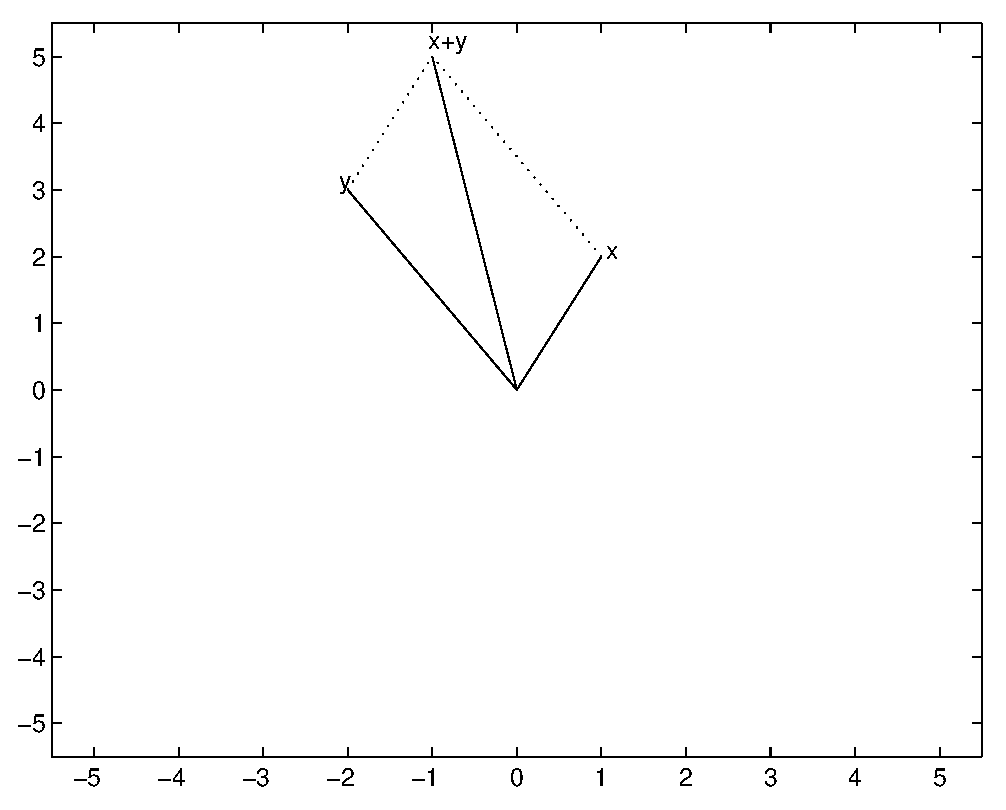
\psfig{file=figures/vec2.eps,width=2.5in}}
         \caption{Addition of two planar vectors.}
         \label{F:vec2}
\end{figure}


The parallelogram law (the diagonal of the parallelogram spanned
by $x$ and $y$ is $x+y$) is equally valid in three dimensions.
Use \Matlab to verify this statement by typing:
\begin{verbatim}
x = [1 0 2];
y = [-1 4 1];
addvec3(x,y)
\end{verbatim} \index{\computer!addvec3}
The parallelogram spanned by $x$ and $y$ in $\R^3$ is shown in
cyan; the diagonal $x+y$ is shown in blue.  See Figure~\ref{F:vec3}.   
To test your geometric intuition, make several choices of vectors $x$ and
$y$.  Note that one vertex of the parallelogram is always the
origin.

\begin{figure}[htb]
         \centerline{%
         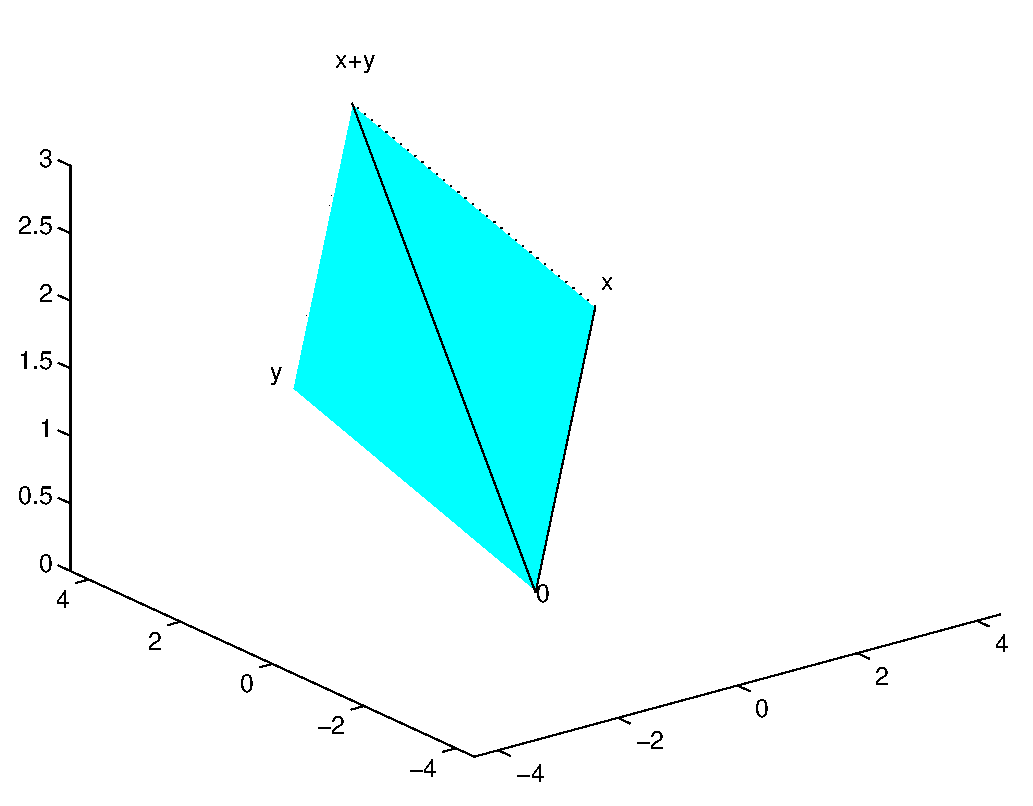
\psfig{file=figures/vec3.eps,width=3.0in}}
         \caption{Addition of two vectors in three dimensions.}
         \label{F:vec3}
\end{figure}


\subsection*{Geometry of Scalar Multiplication}

In all dimensions scalar multiplication\index{scalar
multiplication} just scales the length of the vector.  To
discuss this point we need to define the length of a vector.
View an $n$-vector $x=(x_1,\ldots,x_n)$ as a line segment from
the origin to the point $x$.  Using the Pythagorean theorem, it can
be shown that the {\em length\/}\index{length}\index{vector!length} 
or {\em norm\/}\index{norm}\index{vector!norm} of this line segment is:
\[
||x||  = \sqrt{x_1^2 + \cdots + x_n^2}.
\] \index{\computer:$||\cdot|| $}
\Matlab has the command {\tt norm} for finding the length of a
vector.  Test this by entering the $3$-vector
\begin{verbatim}
x = [1 4 2];
\end{verbatim}
Then type
\begin{verbatim}
norm(x)
\end{verbatim}  \index{\computer!norm}
\Matlab responds with:
\begin{verbatim}
ans =
    4.5826
\end{verbatim}
which is indeed approximately $\sqrt{1+4^2+2^2} = \sqrt{21}$.

Now suppose $r\in\R$ and $x\in\R^n$.  A calculation shows that
\begin{equation}  \label{E:lengths}
||rx||  = |r| ||x||.
\end{equation}
See Exercise~\ref{c1.4.9A}.  Note also that if $r$ is positive, 
then the direction of $rx$
is the same as that of $x$; while if $r$ is negative, then the
direction of $rx$ is opposite to the direction of $x$.  The
lengths of the vectors $3x$ and $-3x$ are each three times the
length of $x$ --- but these vectors point in opposite
directions.  Scalar multiplication by the scalar $0$ produces
the $0$ vector, the vector whose entries are all zero.

\subsection*{Dot Product and Angles}

The {\em dot product\/}\index{dot product} of two $n$-vectors
$x=(x_1,\ldots,x_n)$ and $y=(y_1,\ldots,y_n)$ is an important
operation on vectors.  It is defined by:
\begin{equation}  \label{e:dotproduct}
x\cdot y = x_1y_1 + \cdots + x_ny_n.
\end{equation}
Note that $x\cdot x$ is just $||x||^2$, the length of $x$
squared.

\Matlab also has a command for computing dot products of
$n$-vectors.  Type
\begin{verbatim}
x = [1 4 2];
y = [2 3 -1];
dot(x,y)
\end{verbatim}\index{\computer!dot}
\Matlab responds with the dot product of $x$ and $y$, namely,
\begin{verbatim}
ans =
    12
\end{verbatim}

One of the most important facts concerning dot products is the
one that states
\begin{equation} \label{dotprod=0}
x\cdot y = 0 \quad \mbox{if and only if} \quad \mbox{$x$ and $y$
are perpendicular}.
\end{equation}  \index{perpendicular}
Indeed, dot product also gives a way of numerically determining
the angle between $n$-vectors, as follows.
\begin{thm} \label{T:dotangle}
Let $\theta$ be the angle between two nonzero $n$-vectors $x$
and $y$.  Then
\begin{equation}  \label{e:dotproductang}
\cos \theta = \frac{x\cdot y}{||x|| ||y||}.
\end{equation}
\end{thm}
It follows that $\cos \theta=0$
if and only if $x\cdot y = 0$.  Thus \Ref{dotprod=0} is valid.

\proof  Theorem~\ref{T:dotangle} is just a restatement of the
{\em law of cosines\/}\index{law of cosines}.  Recall that the
law of cosines states that
\[
c^2 = a^2 + b^2 -2ab\cos\theta,
\]
where $a,b,c$ are the lengths of the sides of a triangle and $\theta$
is the interior angle opposite the side of length $c$.
In vector notation we can form a triangle two of whose sides are
given by $x$ and $y$ in $\R^n$.  The third side is just $x-y$ as
$x=y+(x-y)$, as in Figure~\ref{F:costri}.

\begin{figure}[htb]
     \centerline{%
     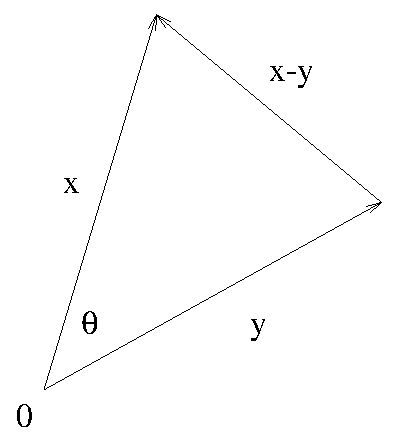
\psfig{file=figures/costri.eps,height=2.0in}}
     \caption{Triangle formed by vectors $x$ and $y$ with interior
	angle $\theta$.}
     \label{F:costri}
\end{figure}

It follows from the law of cosines that
\[
||x-y||^2 = ||x||^2 + ||y||^2 - 2||x|| ||y||  \cos\theta.
\]
We claim that
\[
||x-y||^2 = ||x||^2 + ||y||^2 -2x\cdot y.
\]
Assuming that the claim is valid, it follows that
\[
x\cdot y = ||x|| ||y||  \cos\theta,
\]
which proves the theorem.  Finally, compute
\begin{eqnarray*}
||x-y||^2 & = &(x_1-y_1)^2 + \cdots + (x_n-y_n)^2 \\
& = & (x_1^2-2x_1y_1+y_1^2) + \cdots + (x_n^2-2x_ny_n+y_n^2)\\
& = & (x_1^2+\cdots+x_n^2)-2(x_1y_1+\cdots+x_ny_n)+(y_1^2+\cdots+y_n^2)\\
& = & ||x||^2 -2x\cdot y + ||y||^2
\end{eqnarray*}
to verify the claim.   \qed

Theorem~\ref{T:dotangle} gives a numerically efficient method
for computing the angle\index{angle between vectors} between
vectors $x$ and $y$.  In \Matlab
this computation proceeds by typing
\begin{verbatim}
theta = acos(dot(x,y)/(norm(x)*norm(y)))
\end{verbatim} \index{\computer!acos}\index{\computer!dot}
where {\tt acos} is the inverse cosine of a number.
For example, using the $3$-vectors $x = (1,4,2)$ and $y =
(2,3,-1)$ entered previously, \Matlab responds with
\begin{verbatim}
theta =
    0.7956
\end{verbatim}
Remember that this answer is in radians\index{radians}.  To convert
this answer to degrees\index{degrees}, just multiply by $360$ and
divide by $2\pi$:
\begin{verbatim}
360*theta / (2*pi)
\end{verbatim}
to obtain the answer of $45.5847^\circ$.

\subsubsection{Area of Parallelograms}

Let $P$ be a parallelogram whose sides are the vectors $v$ and $w$ as
in Figure~\ref{F:parallel}.  Let $|P|$ denote the area of $P$.  As an
application of dot products \index{dot product} and
\Ref{e:dotproductang}, we calculate $|P|$. \index{parallelogram}
We claim that
\begin{equation}  \label{e:areaP}
|P|^2 = ||v||^2||w||^2 - (v\cdot w)^2.
\end{equation}
We verify \Ref{e:areaP} as follows.  Note that the area of $P$
is the same as the area of the rectangle $R$ also pictured in
Figure~\ref{F:parallel}.  The side lengths of $R$ are: $||v||$ and
$||w||\sin\theta$ where $\theta$ is the angle between $v$ and $w$.
A computation using \Ref{e:dotproductang} shows that
\begin{eqnarray*}
|R|^2 & = & ||v||^2 ||w||^2\sin^2\theta \\
& = & ||v||^2 ||w||^2(1-\cos^2\theta) \\
& = & ||v||^2 ||w||^2\left(1-\left(\frac{v\cdot w}{||v|| ||w||}
\right)^2\right)\\
& = & ||v||^2 ||w||^2 - (v\cdot w)^2,
\end{eqnarray*}
which establishes \Ref{e:areaP}.

\begin{figure}[htb]
     \centerline{%
     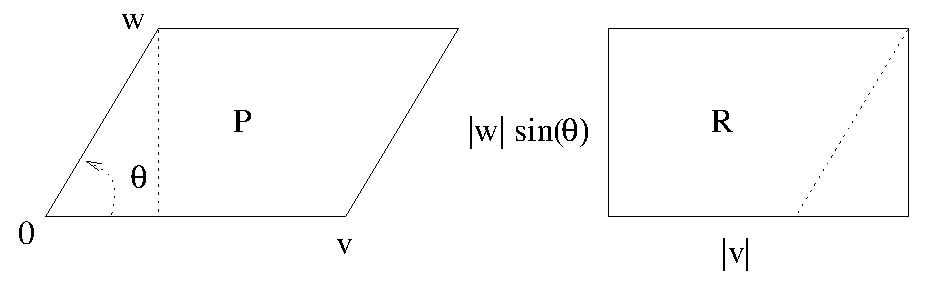
\psfig{file=figures/parallel.eps,width=3.5in}}
     \caption{Parallelogram $P$ beside rectangle $R$ with same area.}
     \label{F:parallel}
\end{figure}


\EXER

\TEXER

\noindent In Exercises~\ref{c1.4.8a} -- \ref{c1.4.8d}
compute the lengths of the given vectors.
\begin{exercise} \label{c1.4.8a}
$x=(3,0)$.
\end{exercise}
\begin{exercise} \label{c1.4.8b}
$x=(2,-1)$.
\end{exercise}
\begin{exercise} \label{c1.4.8c}
$x=(-1,1,1)$.
\end{exercise}
\begin{exercise} \label{c1.4.8d}
$x=(-1,0,2,-1,3)$.
\end{exercise}


\noindent In Exercises~\ref{c1.4.1a} -- \ref{c1.4.1c} determine
whether the given pair of vectors is perpendicular.
\begin{exercise} \label{c1.4.1a}
$x=(1,3)$ and $y=(3,-1)$.
\end{exercise}
\begin{exercise} \label{c1.4.1b}
$x=(2,-1)$ and $y=(-2,1)$.
\end{exercise}
\begin{exercise} \label{c1.4.1bb}
$x=(1,1,3,5)$ and $y=(1,-4,3,0)$.
\end{exercise}
\begin{exercise} \label{c1.4.1c}
$x=(2,1,4,5)$ and $y=(1,-4,3,-2)$.
\end{exercise}


\begin{exercise} \label{c1.4.2}
Find a real number $a$ so that the vectors
\[
x = (1,3,2) \AND y = (2,a,-6)
\]
are perpendicular.
\end{exercise}

\begin{exercise} \label{c1.4.3}
Find the lengths of the vectors $u=(2,1,-2)$ and $v=(0,1,-1)$,
and the angle between them.
\end{exercise}

\noindent In Exercises~\ref{c1.4.9a} -- \ref{c1.4.9f}
compute the dot product $x\cdot y$ for the given pair of vectors and 
the cosine of the angle between them.
\begin{exercise} \label{c1.4.9a}
$x=(2,0)$ and $y=(2,1)$.
\end{exercise}
\begin{exercise} \label{c1.4.9b}
$x=(2,-1)$ and $y=(1,2)$.
\end{exercise}
\begin{exercise} \label{c1.4.9c}
$x=(-1,1,4)$ and $y=(0,1,3)$.
\end{exercise}
\begin{exercise} \label{c1.4.9d}
$x=(-10,1,0)$ and $y=(0,1,20)$.
\end{exercise}
\begin{exercise} \label{c1.4.9e}
$x=(2,-1,1,3,0)$ and $y=(4,0,2,7,5)$.
\end{exercise}
\begin{exercise} \label{c1.4.9f}
$x=(5,-1,4,1,0,0)$ and $y=(-3,0,0,1,10,-5)$.
\end{exercise}

\begin{exercise}  \label{c1.4.9A}
Using the definition of length, verify that formula \Ref{E:lengths} 
is valid.
\end{exercise}


\CEXER

\begin{exercise} \label{c1.4.4}
Use {\tt addvec} and {\tt addvec3} to add vectors in $\R^2$ and
$\R^3$.  More precisely, enter pairs of $2$-vectors {\tt x} and {\tt y} 
of your choosing into \Matlabp, use {\tt addvec} to compute {\tt x+y},
and note the parallelogram formed by $0,x,y,x+y$.  Similarly, enter 
pairs of $3$-vectors and use {\tt addvec3}.
\end{exercise}

\begin{exercise} \label{c1.4.5}
Determine the vector of length $1$ that points in the same direction
as the vector
\[
x=(2,13.5,-6.7,5.23).
\]
\end{exercise}

\begin{exercise} \label{c1.4.5b}
Determine the vector of length $1$ that points in the same direction
as the vector
\[
y=(2.1,-3.5,1.5,1.3,5.2).
\]
\end{exercise}

\noindent In Exercises~\ref{c1.4.6a}-- \ref{c1.4.6c} find the angle in
degrees between the given pair of vectors.
\begin{exercise} \label{c1.4.6a}
$x=(2,1,-3,4)$ and $y=(1,1,-5,7)$.
\end{exercise}
\begin{exercise} \label{c1.4.6b}
$x=(2.43, 10.2,-5.27,\pi)$ and $y= (-2.2,0.33,4,-1.7)$.
\end{exercise}
\begin{exercise} \label{c1.4.6c}
$x=(1,-2,2,1,2.1)$ and $y=(-3.44,1.2,1.5,-2,-3.5)$.
\end{exercise}

\noindent In Exercises~\ref{c1.4.7a} -- \ref{c1.4.7b} let $P$ be the 
parallelogram generated by the given vectors $v$ and $w$ in $\R^3$.  
Compute the area of that parallelogram.
\begin{exercise} \label{c1.4.7a}
$v=(1,5,7)$ and $w=(-2,4,13)$.
\end{exercise}
\begin{exercise} \label{c1.4.7b}
$v=(2,-1,1)$ and $w=(-1,4,3)$.
\end{exercise}
\end{document}
